\documentclass[a4paper,12pt]{article}

\usepackage{./setting/preamble}
 
\begin{document}
\onecolumn
\documentclass[class=article,crop=false,11pt]{standalone}
\usepackage{../setting/preamble_}

\begin{document}
\begin{titlepage}

    \center

    % University
    \textsc{\Large Department of Electronic and Telecommunication}\\[.4cm]
    \textsc{\Large University of Moratuwa}\\[1cm]

    % Document info
    \textsc{\Large EN2090 : LABORATORY PRACTICE-II}\\[0.2cm]
    \textsc{\large }\\[1cm] 										% Course Code
    \HRule \\[0.5cm]
    { \LARGE \bfseries The Analog-Piano}\\[0.3cm]
    \HRule \\[1.5cm]
    \large
    \begin{center}
        \begin{tabular}{l l}
            \multicolumn{2}{c}{\textbf{Team : Dream Epic}} \\\\
            S.Sanjith  & 190562G \\
            T.Sajeepan & 190539T \\
            K.G.C.P.Sandaruwan  & 190557V \\
            G.S.M.U.K.Samarakoon & 190543B \\
        \end{tabular}
    \end{center}
\vspace*{1cm}
    {\Large \today}\\[1cm]
    
\includegraphics[width=0.4\textwidth]{mora.png}\\[1cm] 
    The report is submitted as a partial fulfillment of the module EN2090.\\
    [2cm]
    \HRule\\
    \begin{flushleft}
        \vspace*{-.2cm}
        \emph{Our sincere thanks to Mr.Bhanuka Silva.}
    \end{flushleft}
    \vfill
\end{titlepage}
\end{document}




\tableofcontents
\vspace*{1cm}
All the circuit virtual simulation circuits and results can be found \href{https://github.com/sanjith1999/Analog-Piano.git}{here.}
\vspace*{3cm}
\begin{abstract}
    The electronic pianos available in the markets are using a pre-recorded audio of the sound to generate the tones. The task of this project is explore the possible analog designs to synthesize a tone. In this report, we have discussed our views and experiences on a stable design for synthesizing middle octave c-Note. An audio amplifier design that improvises the generated sound quality and capable of driving mid-power speakers is included in parallel at each stage.
\end{abstract}
\newpage


\twocolumn
\section{Introduction}
Music is one of the key things to please people and it’s based on musical notes. It is so wonderful to observe such notes can be generated by combining electrical signals.
\par
In this device sound of the middle octave, C is mimicked by synthesizing signals. For this purpose, four wien-bridge oscillators have been used to generate sinusoidal waveforms relevant to the major harmonics of the C note. Then these signals are added by a scaling adder and amplified using a Class AB amplifier. A speaker(8$\Omega$ preferred) ranges around 3W could be used with the pinout to observe the sound output. 
\par
The volume of the speaker and the noise level can be adjusted as the user desires. A complete electronic piano can be implemented by combining such modules and changing the essentials accordingly to generate different notes. The following report will elaborate on the experiences and ideas behind the design process.
\documentclass[class=article,crop=false]{standalone}

\usepackage{../setting/preamble_}

\begin{document}
\twocolumn

\section{Theory}
\subsection{Oscillator}
\begin{wrapfigure}{l}{0.3\columnwidth}
  \vspace*{-.5cm}
  \begin{center}
    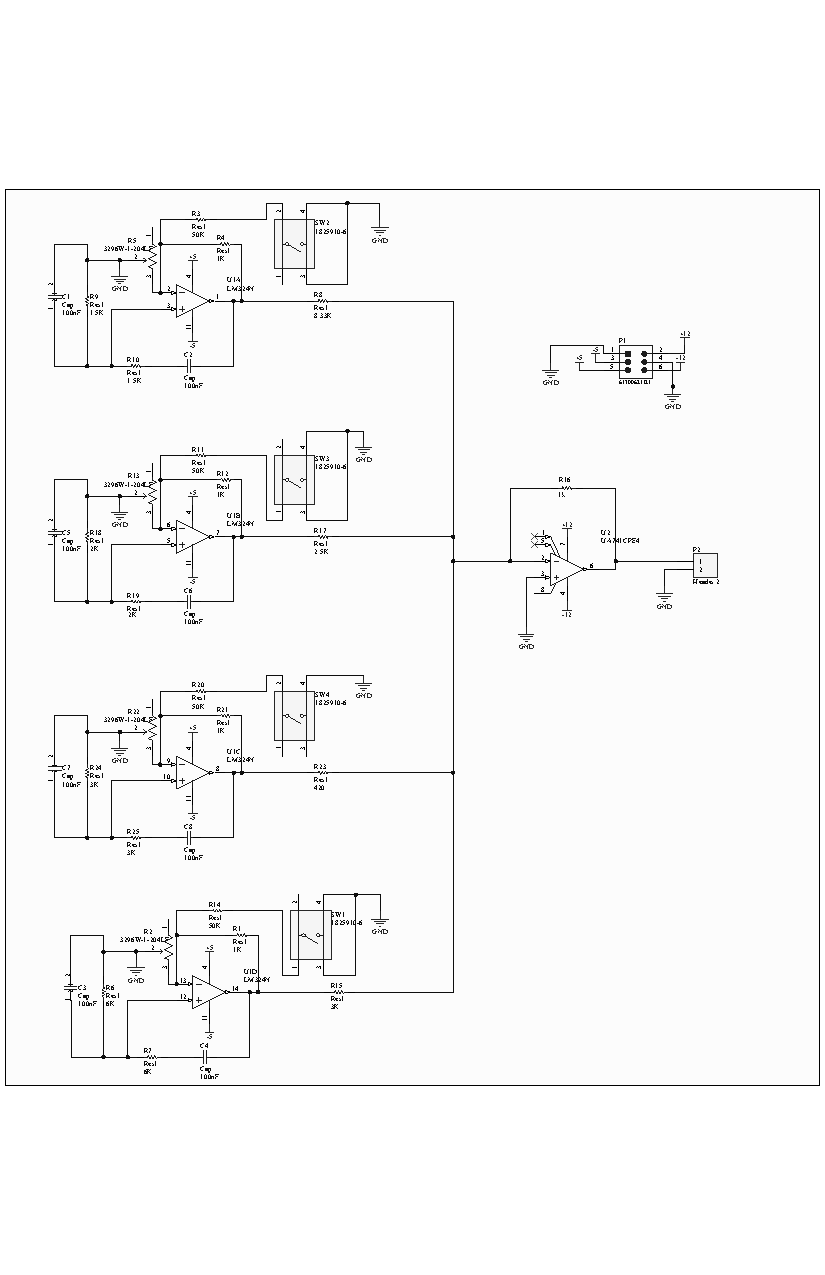
\includegraphics[width=0.3\columnwidth]{oscillator}
  \end{center}
  \vspace*{-.5cm}
\end{wrapfigure}

An oscillator is an amplifier that uses positive feedback that generates an output frequency without the use of an externally applied input signal. Once the oscillation is started, the parameters A and $\beta$ are aligned to maintain a unity gain at the required frequency in order to keep the oscillation indefinitely stable.

\subsubsection*{Wein-Bridge Oscillator}
The Wien Bridge Oscillator uses a feedback circuit consisting of a series RC node cascaded with a parallel RC of the same component values producing a phase delay or phase advance circuit depending upon the frequency. Effectively they act as a second-order frequency dependant Band-Pass-Filter with a high Q factor at the selected frequency $f_r=\frac{1}{2\pi RC}$. This RC network is connected in the positive feed-back path of the amplifier and has zero phase shift at just one frequency.
\par
Other part of the feedback signal is connected to the inverting input terminal(negative feed-back) via resistor divider network of $R_1\&R_2$.Then at the selected resonant frequency($f_r$), the voltages applied to the inverting and non-inverting inputs will be equal and “in-phase”. So the positive feedback will cancel out the negative feedback signal causing the circuit to oscillate.

\begin{figure} 
  \begin{subfigure}{.33\columnwidth}
    \centering
    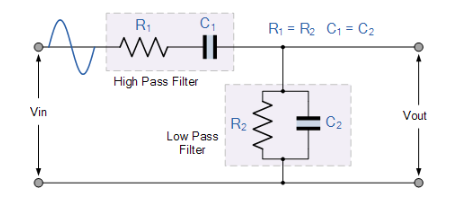
\includegraphics[width=.95\columnwidth]{weistan_1}
    \caption*{RC-Network}  
  \end{subfigure}
  \begin{subfigure}{.33\columnwidth}
    \centering
    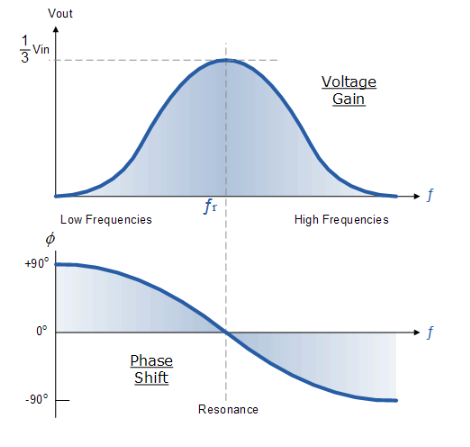
\includegraphics[width=.95\columnwidth]{weistan_2}  
    \caption*{Response}
  \end{subfigure}
  \begin{subfigure}{.3\columnwidth}
    \centering
    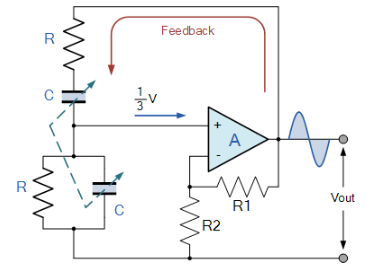
\includegraphics[width=.95\columnwidth]{weistan_3}
    \caption*{Oscillator}  
  \end{subfigure}
\end{figure}
\subsubsection*{Starting and Damping Oscillation}
By controlling the negative feedback ratio($\frac{R_2}{R_1+R_2}$) of the oscillator we can start and damp the oscillation as required. To start oscillation, we need to slightly reduce the negative feedback($<\frac{1}{3}$). This will give rise to a resultant signal on the amplifier input side which is get amplified and fed back recursively turns out to drive oscillation.
\par
Keeping the feedback ratio slightly more($>\frac{1}{3}$) will give rise to a resultant negative input which is get added adversely with output resulting in damping of the oscillation. By fine-tuning the ratio in a very elegant manner, it is possible to control the damping time constant.
\subsection{Amplifier}
Driving a high-power speaker draws a high amount of current from the circuit. These current ranges are very much higher than the maximum supply available from op-amps and other low power components used in generating the wave patterns. So it is crucial to maintain an amplifier boundary between low power noisy signal to high power driving signal free of noise. In the following context, we will discuss the theories behind our amplifier design in detail.
\subsubsection*{Class-A }
\begin{wrapfigure}{l}{0.35\columnwidth}
  \vspace*{-.5cm}
  \begin{center}
    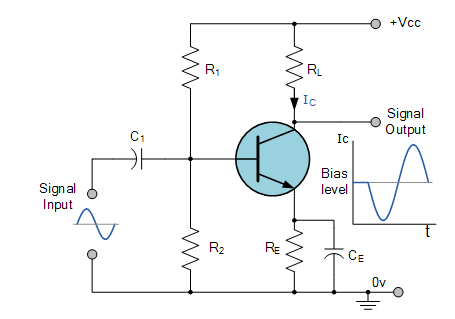
\includegraphics[width=0.35\columnwidth]{classA}
  \end{center}
  \vspace*{-.5cm}
\end{wrapfigure}
These are the simplest configuration among other families. It uses a single-ended transistor for its output stage with the resistive load connected directly to the Collector terminal. When the transistor switches “ON” it sinks the output current through the Collector resulting in an inevitable voltage drop across the Emitter resistance thereby limiting the negative output capability.  
\par 
The current handling capability of such an amplifier family can be increased drastically by replacing the output transistor with \textbf{Darlington pair}. These devices provide high input impedance.
\subsubsection*{Class-B}
Class B Amplifiers are biased to only conduct half of the input signal. Using 2 such amplifiers arranged in a “Push-Pull” configuration, and combining the output signal, the full waveform can be obtained.
\par
As the quiescent current for this amplifier is 0, there is little or no DC, therefore much less power dissipation. However, there is a slight waveform distortion due to the bias voltage requirement of the transistor known as cross-over distortion.
\subsubsection*{Class-AB} 
Class AB amplifiers overcome the distortion issue of class B amplifiers by permanently bringing the two transistors just into the active region. This reduces the efficiency, but results in an undistorted the waveform in the output.
\par
\begin{figure}
  \vspace*{-.7cm}
  \begin{center}
    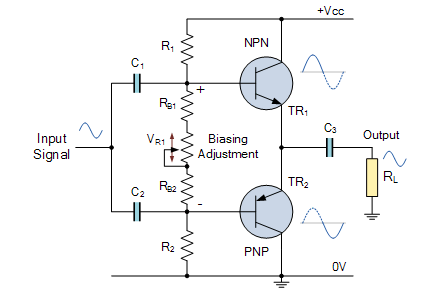
\includegraphics[width=.6\columnwidth]{classAB}
  \end{center}
  \vspace*{-.5cm}
\end{figure}
As the power dissipation due to the DC component is much less than class A amplifiers, these circuits allow the use of compact heat sinks during the operation.
\subsubsection*{Variable Zerner Diode}
\begin{wrapfigure}{r}{0.2\columnwidth}
  \vspace*{-1cm}
  \begin{center}
    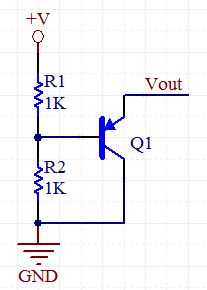
\includegraphics[width=0.2\columnwidth]{zener}
  \end{center}
  \vspace*{-.5cm}
\end{wrapfigure}
This variable Zener diode circuit acts like a Zener diode with a breakdown voltage adjustable in a vast domain. This is achieved by driving a BJT in the active region and controlling the base current. The current through the voltage divider $R_1\&R_2$ must be higher compared to the base current.
\end{document}
\newpage
\documentclass[class=article,crop=false,11pt]{standalone}

\usepackage{../setting/preamble_}

\begin{document}
\twocolumn

\section{Methodology}
\subsection{Preliminary Analysis}
At an earlier stage of the project, we plan to build an octave piano with twelve notes including minor keys. At that stage, we analyzed the frequency spectrum of each note and found out it is possible to produce a majority feeling of sound with only four harmonics to a given note.
\par
After synthesizing all the keynotes from its harmonics using Matlab, we moved to circuit development. At this stage, we decided to stimulate only one note from the piano because the generation of notes is modularizable. For this purpose, we have chosen the C-wave which is in the middle of the spectrum.
\begin{figure}
    \begin{subfigure}{.45\columnwidth}
        \centering
        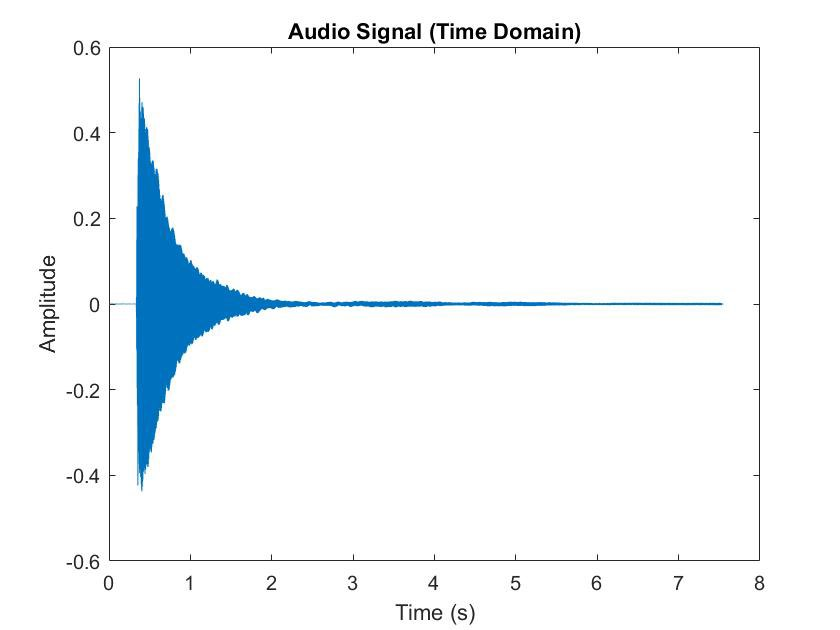
\includegraphics[width=.9\columnwidth]{c_wave}
    \end{subfigure}
    \begin{subfigure}{.45\columnwidth}
        \centering
        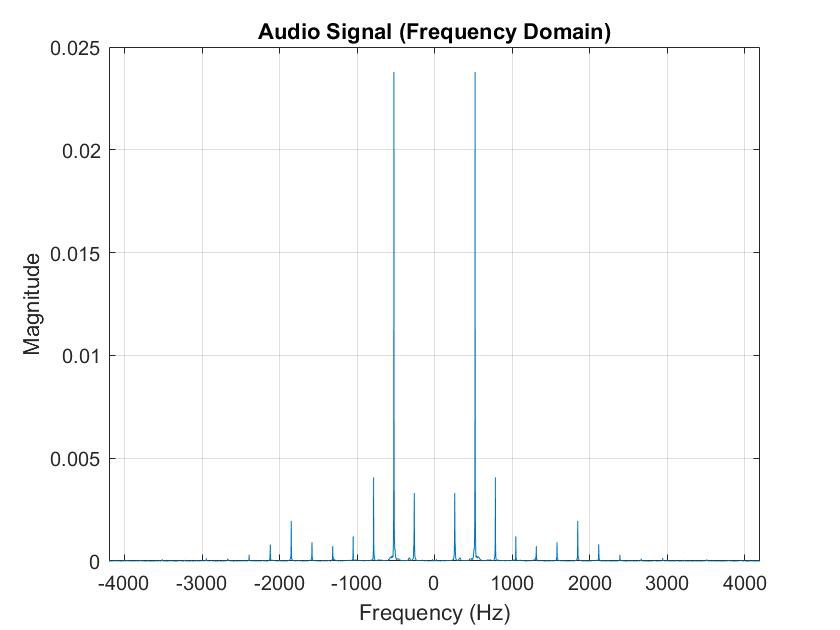
\includegraphics[width=.9\columnwidth]{spectrum_c}
    \end{subfigure}

\end{figure}
\subsection{Circuit Design}

\begin{figure}
    \begin{center}
        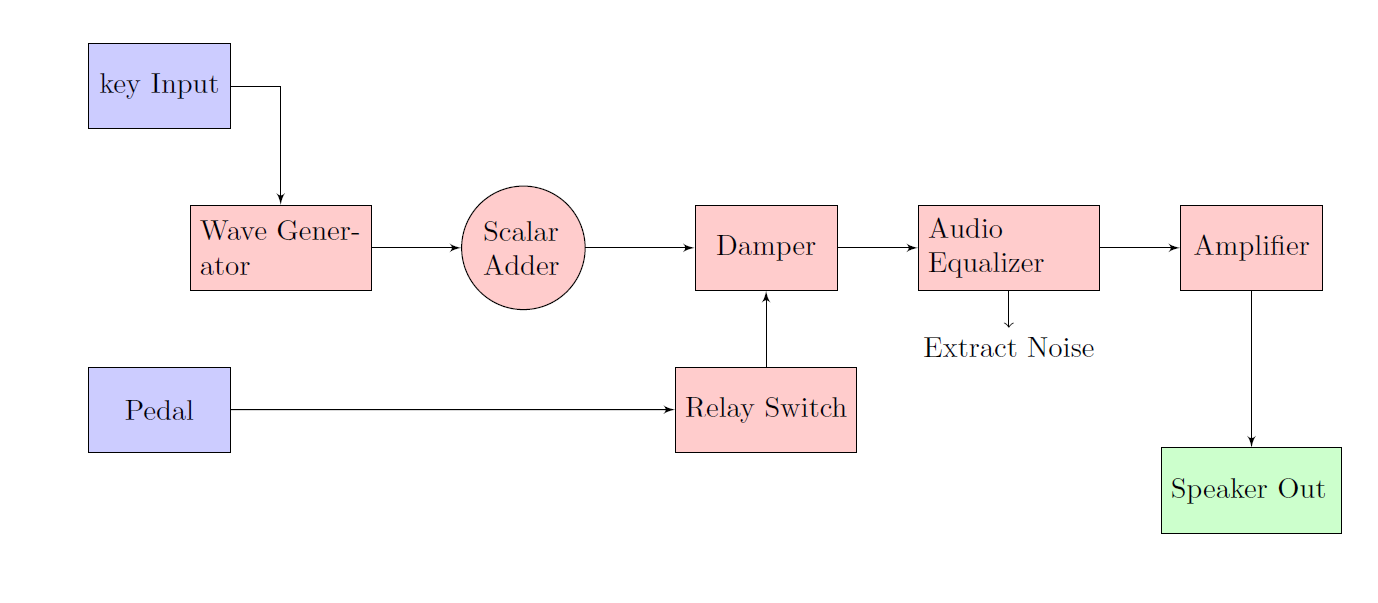
\includegraphics[width=\columnwidth]{flow}
        \caption*{Block Diagram of the Circuit}
    \end{center}
\end{figure}
\subsubsection{Wave Generator}
Square wave generation of half the frequency together with a bandpass active filter is considered in the first stage of the circuit development. Need for achieving a larger Q factor for the filter as the number of harmonics increases, lift the choice to not-feasible.
\par
Moving towards a stable solution brought the Wien bridge oscillator into play. These oscillators have the flexibility over frequency choice ($\frac{1}{2\pi RC}$) making them the most suitable option to be used with modularizable piano.
\subsubsection{Key and Pedal}
\subsubsection{Scalar Adder}
\subsubsection{Amplifier}
At earlier stages, the amplifier was implemented in class-A configuration. The requirement for lower output resistance of the bias path leads to high power dissipation in the signal-free state. This made such a model impossible without larger heatsinks at the cost of low power efficiency.
\begin{figure}
    \begin{center}
        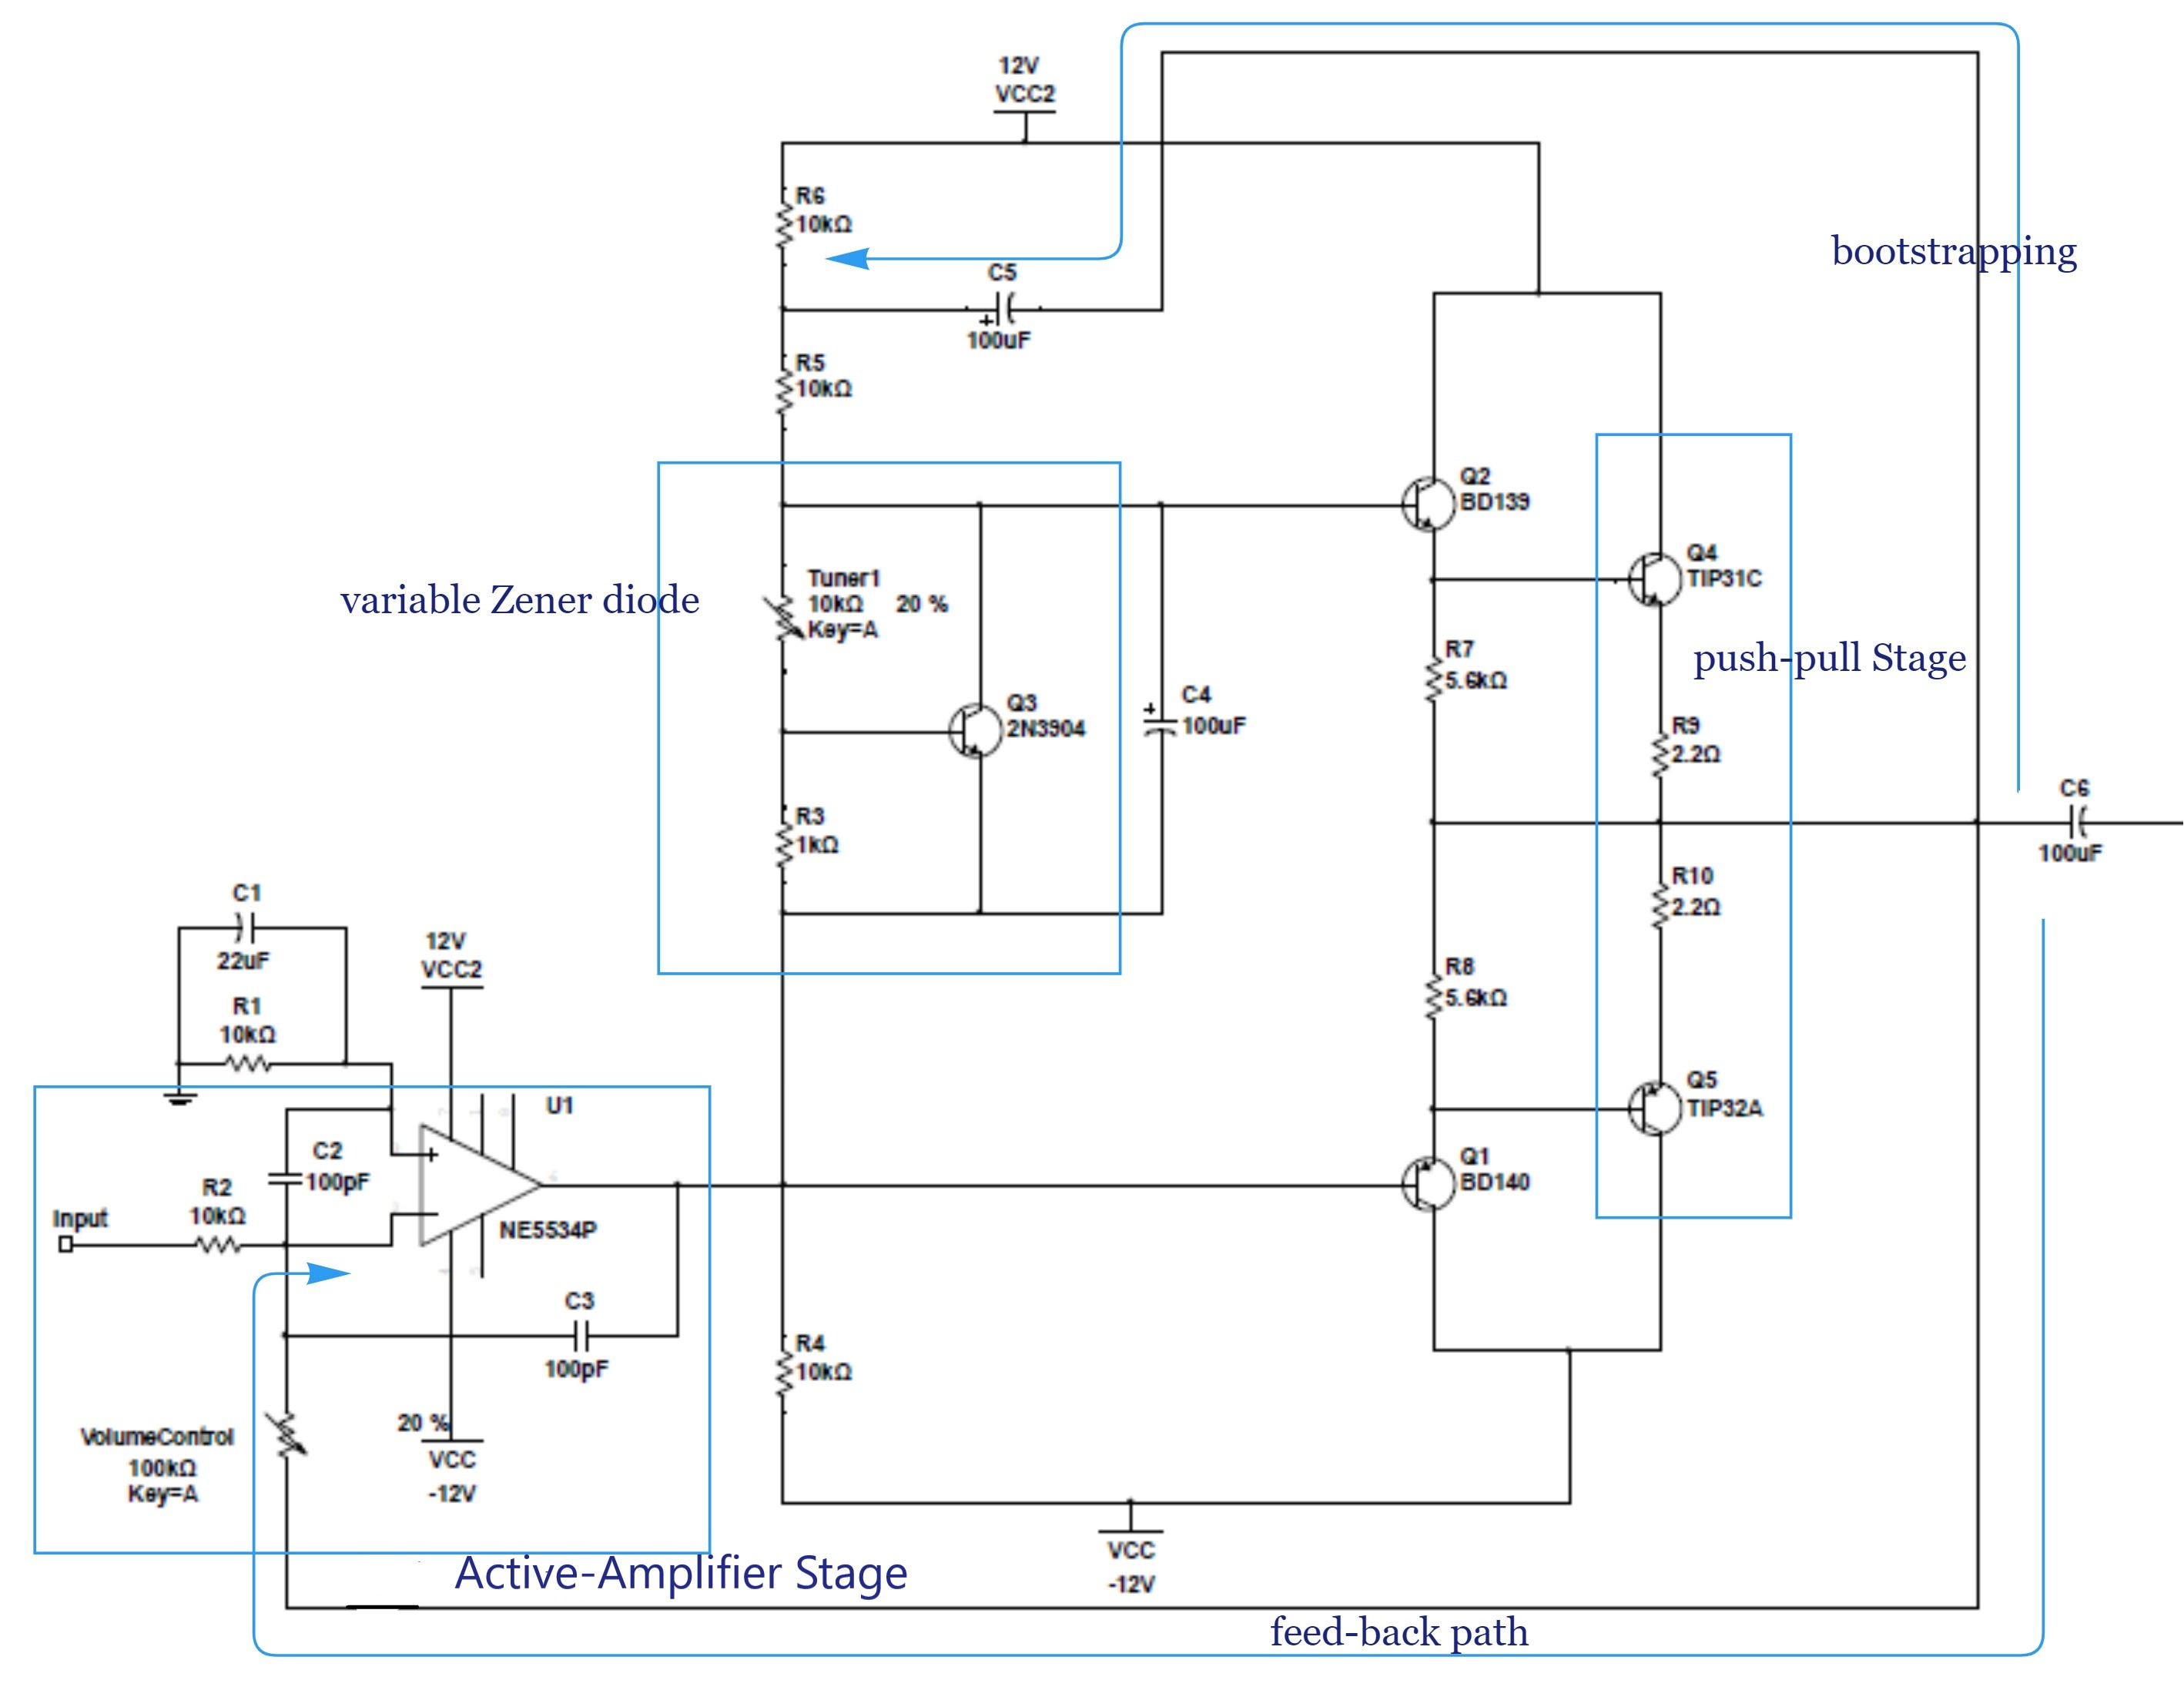
\includegraphics[width=\columnwidth]{amplifier_cd}
    \end{center}
\end{figure}

\textbf{Active Amplifier Stage}: In the first stage of the amplifier an op-amp is used in the inverting-amplifier configuration. The feedback path is connected to the end of the overall circuit to ensure enough current supply available in the output. The op-amp NE5534 was chosen for the purpose according to its key characteristics such as high unity-gain bandwidth(10MHz), low harmonic distortion, and high common-mode rejection ratio (100dB). The values of C2 and C3 are chosen to allow only higher frequencies($>20kHz$) to pass through. These are utilized in a manner to remove high-frequency noises from the wave-form.
\\
\textbf{Push-Pull Stage}: Considering the requirement of high power gain it is decided to engage Darlington pairs for this purpose. These components failed in the long run due to the inability of compensating for high power dissipation. Considering this, the design moved to engage two coupled BJTs to allow the choices for transistors to be used in the high current path. The similar pairs TIP31C and TIP32C were chosen after considering their high power compensation capability(around 40W).
\\
\textbf{Bias}: Due to the requirement for a sudden supply of high current on the keypress, the signal gets noisy when we drive the speaker without any bias. In earlier stages, a few diodes are used to bias the circuit which failed to get rid of the noise. As the next step, we used Zener diodes that provide the capability to choose higher bias voltage. This results in the low efficiency of the circuit.
After considering all the methods it is decided to implement the variable Zener diode which has the flexibility over varying bias voltage in a wider range. This provides control over two extremities, effecieny and quality of the output.
\\
\textbf{Bootstrapping}: The capacitor C5 gets charged to the pre-decided bias voltage.  By maintaining the circuit time constant very large ($t=R5\parallel R6\star C5>0.5S$) the overall bias voltage of the circuit is maintained as a constant value to compensate for the effect of thermal runaway.
\end{document}
\newpage
\section{Results}
The evaluation of the model happened in three stages. The first part completely relied on simulation results. The second was the physical simulation of separate modules independently on the breadboard. Finally, the complete prototype was built and tested.
\par
The requirements that needed to be met, and the
the method utilized to test whether they have been met
are as follows:

\begin{figure}[h]
    \resizebox{\columnwidth}{!}{
        \begin{tabular}{|c|c|c|}
            \toprule
            Design              & \multirow{2}{*}{Target Value} & \multirow{2}{*}{Testing Method}          \\
            Requirement         &                               &                                          \\
            \midrule\midrule
            Spectrum            & Specified Amplitude Ratios    & \multirow{3}{*}{Stimulation}             \\
            \cmidrule(lr){1-2}
            Wave pattern        & Exponential-Decay             &                                          \\
            \cmidrule(lr){1-2}
            Power Efficiency    & 75\%                          &                                          \\
            \midrule
            Speakers            & 4$\Omega$-16$\Omega$ \& 1W-5W & Prototype                                \\
            \midrule
            Quality \& Loudness & 40dB-75dB                     & \multirow{2}{*}{Stimulation/ Prototype } \\
            \cmidrule(lr){1-2}
            Datasheet           & parameters                    &                                          \\
            \bottomrule
        \end{tabular}}
\end{figure}
\subsection{Simulation}
\subsubsection*{Wave Generator}
The outputs of oscillators are very stable although a slight variation in the frequencies($\pm 3$) was observed. The following figures illustrate the observed decay pattern and stable waveform from an oscillator.
\begin{figure}[h]
    \begin{subfigure}{.48\columnwidth}
        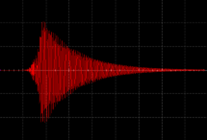
\includegraphics[width=.8\columnwidth]{wave_sim}
        \caption*{Envelope Pattern}
    \end{subfigure}
    \begin{subfigure}{.48\columnwidth}
        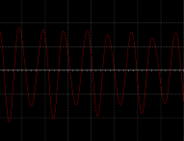
\includegraphics[width=\columnwidth]{s_wave_sim}
        \caption*{Wave Pattern}
    \end{subfigure}
\end{figure}

The output of the scalar adder looked similar to the original waveform and the spectrums were closely matched. Somehow at the simulation stage, sound outputs failed to match. Expected and observed wave characteristics as follows
\begin{figure}[h]
    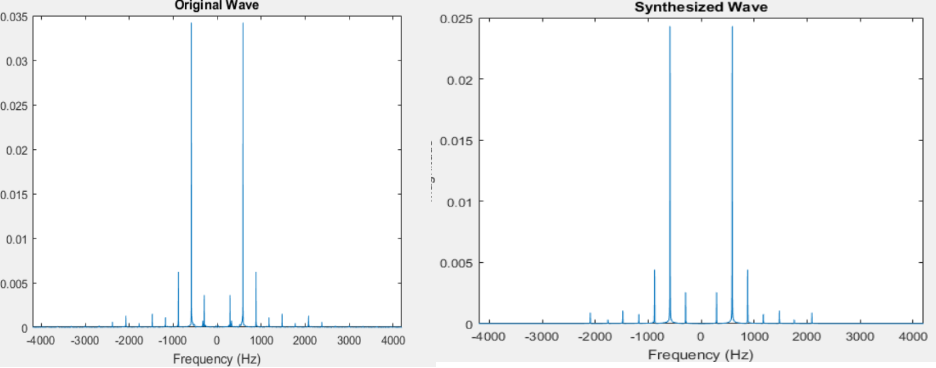
\includegraphics[width=\columnwidth]{spectrum}
\end{figure}
These stages are operated at low power and the oscillations are normally in a damped state. This allows keeping the overall output of the wave generator to be in a normally-off state which is crucial for power efficiency.
\subsubsection*{Amplifier}
Although the wave synthesis process is limited to frequencies lower than 5kHz, it is initially planned to implement an amplifier that has a constant gain throughout the full audible range(up to 20000kHz). From the observations, the model was limited to 12kHz which is expected due to imperfections in transistor behaviors.
\begin{figure}[h]
    \begin{subfigure}{.48\columnwidth}
        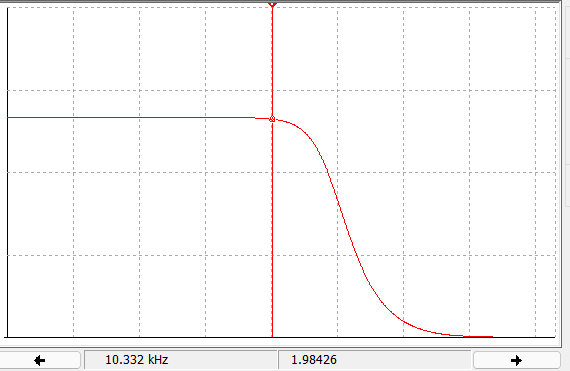
\includegraphics[width=.8\columnwidth]{magnitude}
        \caption*{Voltage Gain}
    \end{subfigure}
    \begin{subfigure}{.48\columnwidth}
        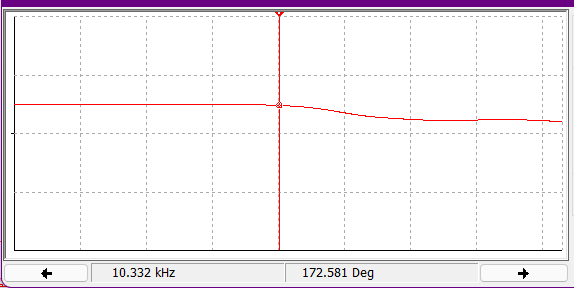
\includegraphics[width=\columnwidth]{phase}
        \caption*{Phase}
    \end{subfigure}
\end{figure}
\\
From the simulation, it was confirmed that the feedback resistance gives linear control over the gain of the amplifier.
\begin{enumerate}
    \item \textbf{Input Resistance} : \textbf{28.2k$\Omega$}\\The input resistance was determined by using the multimeter tool to measure the current drawn from the source and dividing the source voltage by the measured value.
    \item \textbf{Output Impedance} : \textbf{1.9$\Omega$}\\The output impedance was calculated by using voltmeter tool and constant current source. The input was sort-circuited and constant current source applied in the output. Then the voltmeter reading in the current source was measured.
          $$R_{out}=\frac{V_{read}}{I_{source}}$$
    \item \textbf{Bandwidth} : \textbf{200Hz-12kHz}\\Bandwidth was determined using the bode-plot of the amplifier. The region where gain stays constant is only considered.
    \item \textbf{Gain}(8$\Omega$) : \textbf{50dB-70dB}\\The gain was determined using the wattmeter tool between the input source and speaker input.
    \item \textbf{Power Efficiency} : \textbf{69\%}\\
          $$\eta=\frac{P_L}{P_S}\times 100\%$$
    \item \textbf{Safety Measurements :} \\
          The maximum current path was observed to conduct 600mA in the worst case. This was considered in the maximum power calculations and component selections.
\end{enumerate}

\subsection{Circuit Blocks}
\subsubsection*{Wave Generator}
Noise-free stable wave pattern is observed at each oscillator. The measured frequencies vary in the range of 10Hz as expected due to the imperfection in resistance selection. Although the wave pattern observed had  clipping effect it was observed that they could be eliminated by fine-tuning.
\begin{figure}[h]
    \begin{subfigure}{.48\columnwidth}
        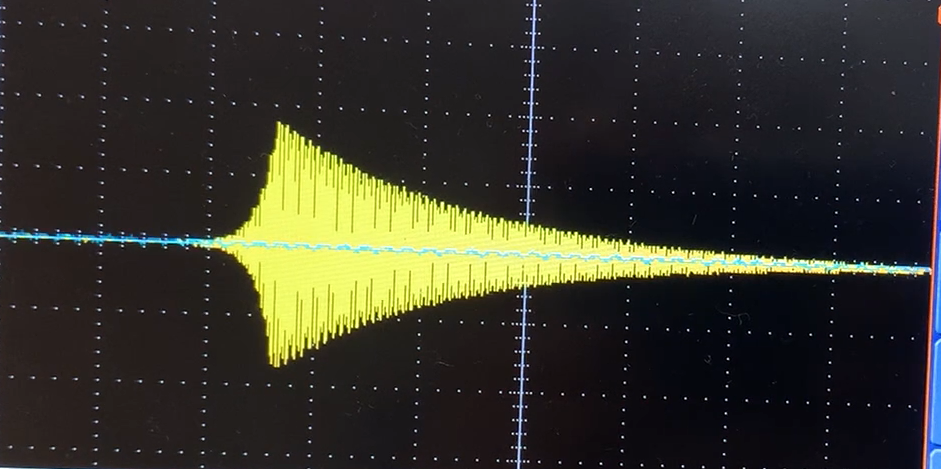
\includegraphics[width=\columnwidth]{wein_phy_2}
        \caption*{Envelope Pattern}
    \end{subfigure}
    \begin{subfigure}{.48\columnwidth}
        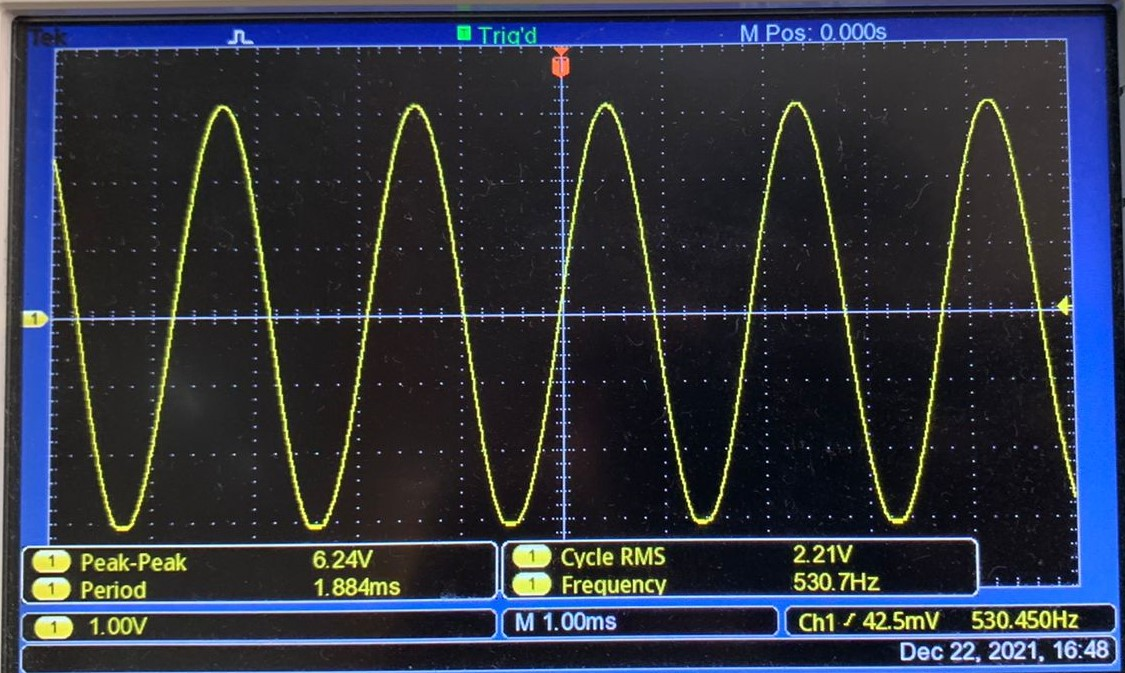
\includegraphics[width=.8\columnwidth]{wein_phy}
        \caption*{Wave Pattern}
    \end{subfigure}
\end{figure}

\subsubsection*{Amplifier}
The parameters measured were varied with simulation results.
\begin{enumerate}
    \item \textbf{Input Resistance} : \textbf{43M$\Omega$}\\The input impedance was determined by using a digital multimeter to measure the current being drawn from the input for an audio input of 0.1mA (peak to peak), with the output open-circuited.
    \item \textbf{Output Impedance} : \textbf{10$\Omega$}\\Output impedance was measured using the voltmeter, from the open circuit reading in the output terminal ($V_O$) and the reading in the 8$\Omega$ load ($V_L$).
          $$R_{out}=R_L\times\frac{V_L}{V_O}$$
    \item \textbf{Bandwidth} : \textbf{200Hz-12kHz}\\Bandwidth was determined using the bode-plot of the amplifier. The region where gain stays constant is only considered.
    \item \textbf{Power Efficiency} : \textbf{63\%}\\
          Efficiency was determined by inspecting the supply and speaker inputs.
    \item \textbf{Maximum Current} : \textbf{0.4mA}
\end{enumerate}
The performance of the amplifier with song output from a mobile phone is also inspected at this stage. The results are as follows.
\begin{figure}[h]
    \includegraphics[width=\columnwidth]{song}
    \caption*{Song Wave : Input - Yellow \& Output - Blue}
\end{figure}

\subsection{Integrated-Circuit}
The wave generator is cascaded with the amplifier to create the final prototype of the design. The sound output of the completed circuit was observed very familiarly with the c-wave of the piano. The waveforms of the original wave and finely tuned wave output are as follows:
\begin{figure}[h]
    \begin{subfigure}{.48\columnwidth}
        \centering
        \includegraphics[width=.9\columnwidth]{c_original_expectation}
        \caption*{Original Wave}
    \end{subfigure}
    \begin{subfigure}{.48\columnwidth}
        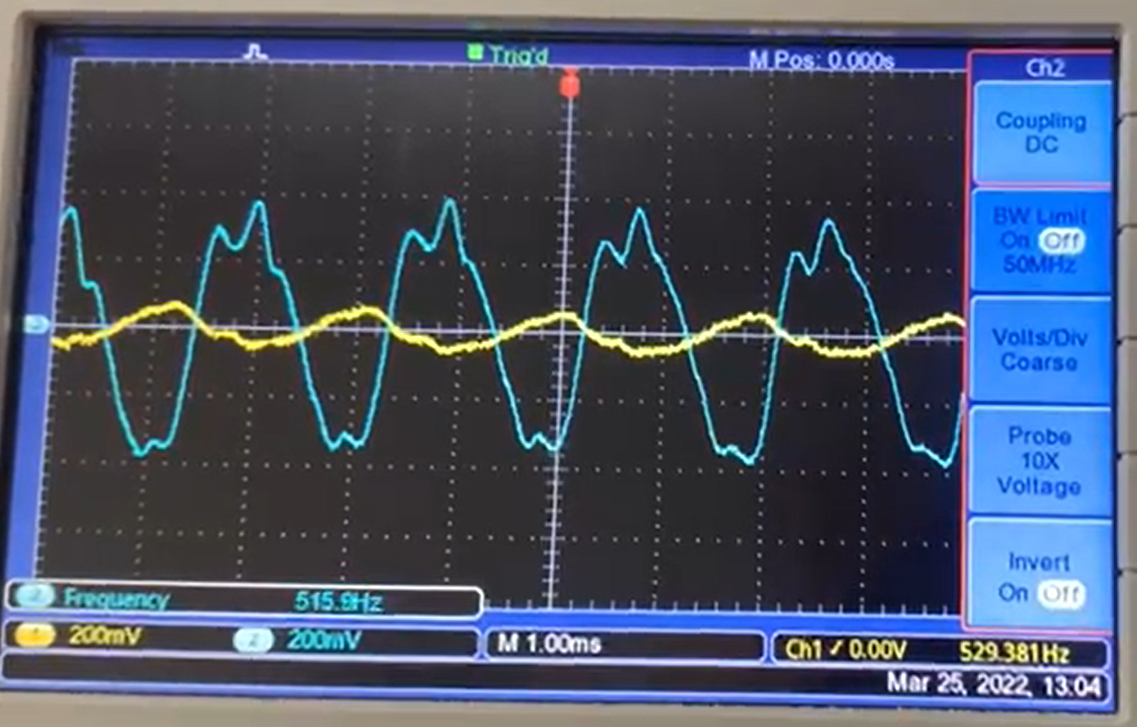
\includegraphics[width=.8\columnwidth]{o_wave_o}
        \caption*{Tuned Output}
    \end{subfigure}
    \begin{subfigure}{\columnwidth}
        \centering
        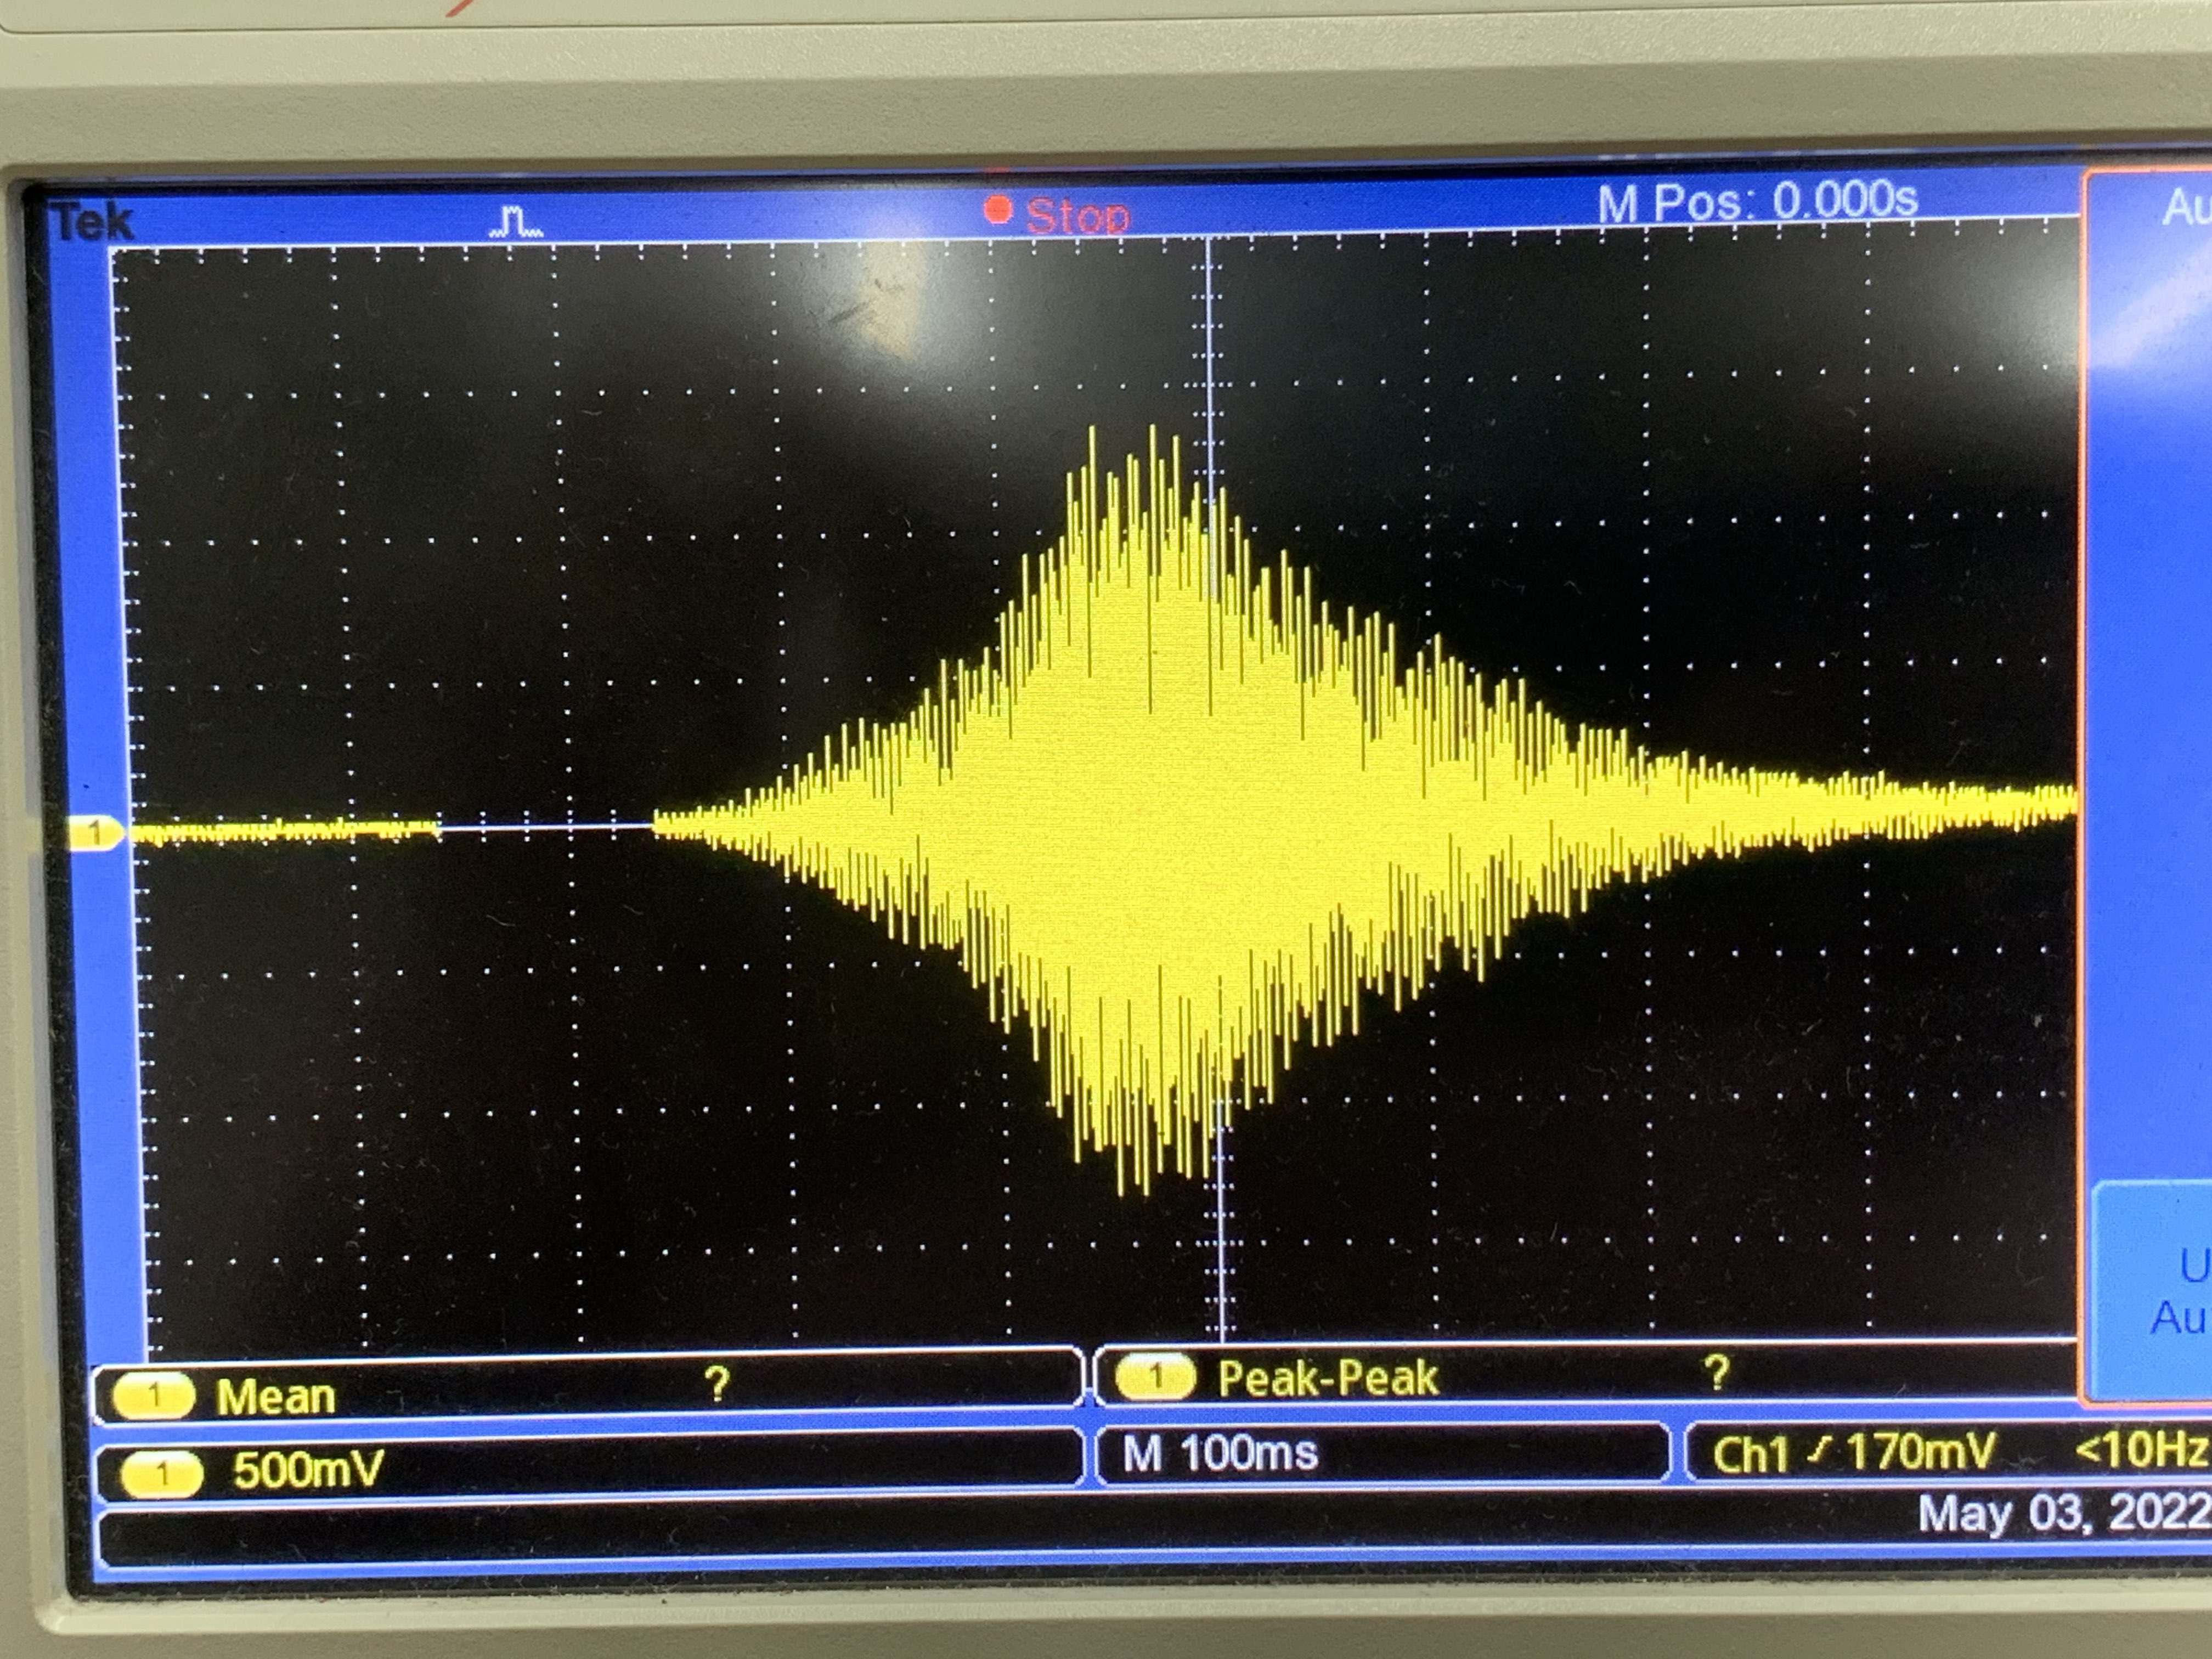
\includegraphics[width=.75\columnwidth]{final_wave}
        \caption*{Envelope Pattern}
    \end{subfigure}
\end{figure}
Although a small elongation was observed at the start of oscillation this could also be controlled by parallel resistance that is responsible for the start of the oscillation. We suspected this behavior is due to an increase in impedance imposed by tracks.
\section{Conclusion}
We were able to complete the project within the given period. Most of the design expectations were achieved. From stable output waves from oscillator up to scaling of each harmonic in the spectrum were finely aligned with expectation. The stability in the gain of the output from the amplifier was adapted even in the situations of thermal-run-away. A better quality equalized sound is accomplished as the overall exploration of the project. 
\par
However, some of the design parameters could not be fully met. The phases of each harmonics could not be able to control rather than fine-tuning the oscillator gains. The amplifier design does not meet the expected efficiency and bandwidth range. While it meets the lower cutoff requirement, the upper cutoff is lower than(12kHz) expectation(20kHz). The best-achieved envelope pattern had elongation in the beginning. The final prototype on the PCB couldn't be able to complete due to the poor quality of the tracks.
\subsection*{Discussion}
\begin{itemize}
    \item Although the wave generator did a fine job with synthesizing c-wave, too many tuning parameters and complexity in combining oscillators make it hard to achieve such a feasible end-product as complete piano with this strategy.
    \item There is a large amount of heat dissipated by the TIP transistors. Heat sinks attached to them failed to compensate for enough heat in the longer run. Thermal-run-away behavior was observed which hindered circuit performance with time. 
    \item The values obtained by the virtual simulation did not agree with the values obtained through the physical prototype. However, the specification sheet has been based on the prototype values. Therefore, the specification sheet will be an accurate representation of the performance.
\end{itemize}
\onecolumn
\section*{References}
\begin{enumerate}
    \item \href{https://web.eecs.utk.edu/~hqi/ece505/project/proj1.pdf}{Synthesis of Musical Notes andInstrument Sounds with Sinusoids}
    \item \href{https://electronics.stackexchange.com/questions/178975/is-it-feasible-to-synthesise-sound-with-analog-circuitry-these-days}{Feasiblity about synthesizing sound with analog
              circuitry}
    \item \href{http://www.vibrationdata.com/piano.htm}{Original Sounds of Piano}
    \item \href{https://universe-review.ca/R12-03-wave02.htm}{Wave, Sound, and Music}
    \item  \href{https://en.wikipedia.org/wiki/Wien_bridge_oscillator}{Weinbridge-Oscillator}
    \item \href{https://www.homemade-circuits.com/simple-sine-wave-generator-circuits/}{Alternative sine wave generators}
    \item \href{https://www.ams.jhu.edu/dan-mathofmusic/sound-waves/}{Mathematics behind wave manipulation}
    \item \href{http://www.jiisuki.net/reports/howto-build-analog-synth.pdf}{How to Design and Build an Analog Synthesizer from Scratch}
\end{enumerate}
\vspace*{5cm}
\section*{Contribution}
\begin{tabular}{|l|l|l|}
    \toprule
    ID NO                    & Member                              & Contribution                                           \\
    \midrule\midrule
    \multirow{2}{*}{190562G} & \multirow{2}{*}{S.Sanjith}          & Damper Design, Improvisation of Amplfier Design,       \\
                             &                                     & Routing of PCBs, Data Sheet Design                     \\
    \midrule
    \multirow{2}{*}{190557V} & \multirow{2}{*}{K.G.C.P.Sandaruwan} & Oscillator Design, Scalar Adder Design                 \\
                             &                                     & Oscillator Schematic Design                            \\
    \midrule
    \multirow{2}{*}{190539T} & \multirow{2}{*}{T.Sajeepan}         & Analyzation of Original Wave, Amplifier Design(basic), \\
                             &                                     & Amplifier schematic design                             \\
    \midrule
    190543B                  & G.S.M.U.K.Samarakoon                & Contribution to Amplifier Design                       \\
    \bottomrule
\end{tabular}
\newpage
\appendix
\section{Circuit Design}
\subsection*{Wave Generator}
\begin{figure}[h]
    \centering
    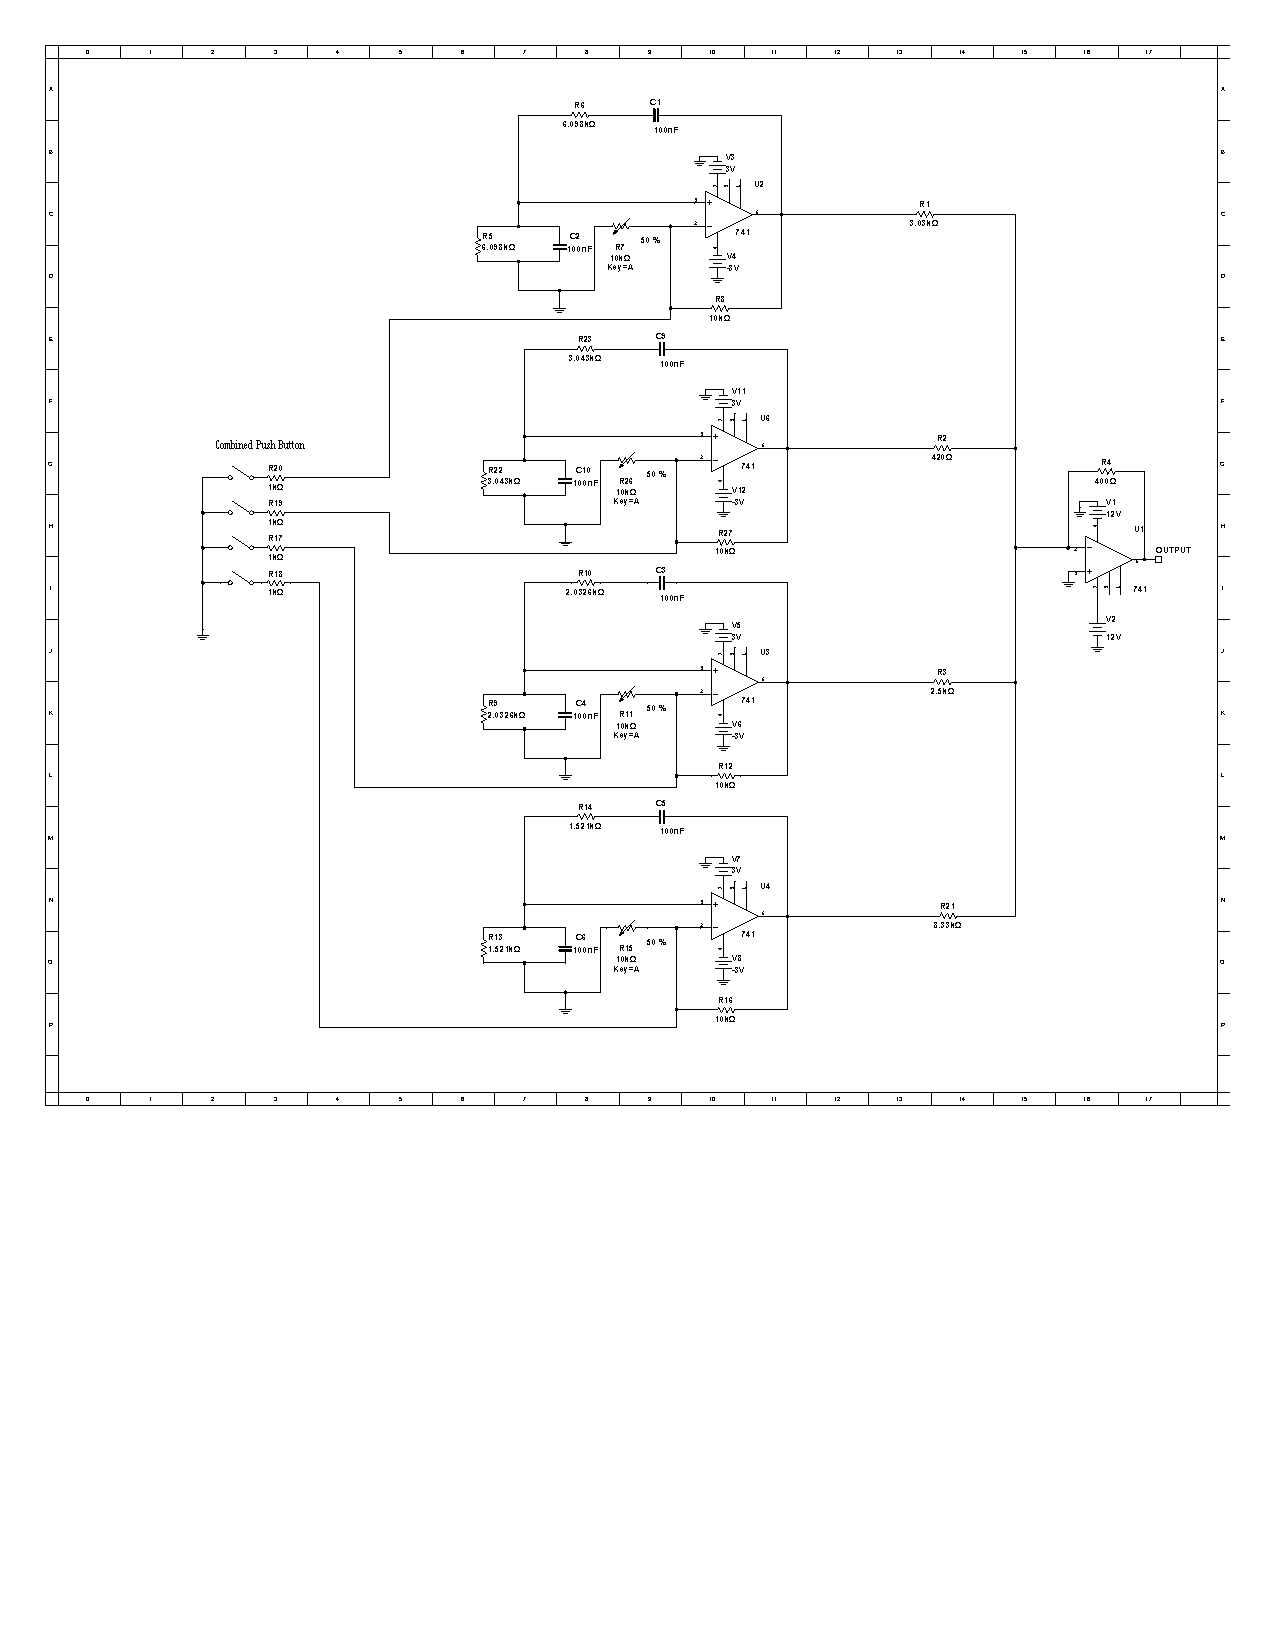
\includegraphics[width=.65\textwidth]{oscillator_mul}
    \vspace*{-5cm}
\end{figure}
\subsection*{Amplifier}
\begin{figure}
    \centering
    \vspace*{-6.5cm}
    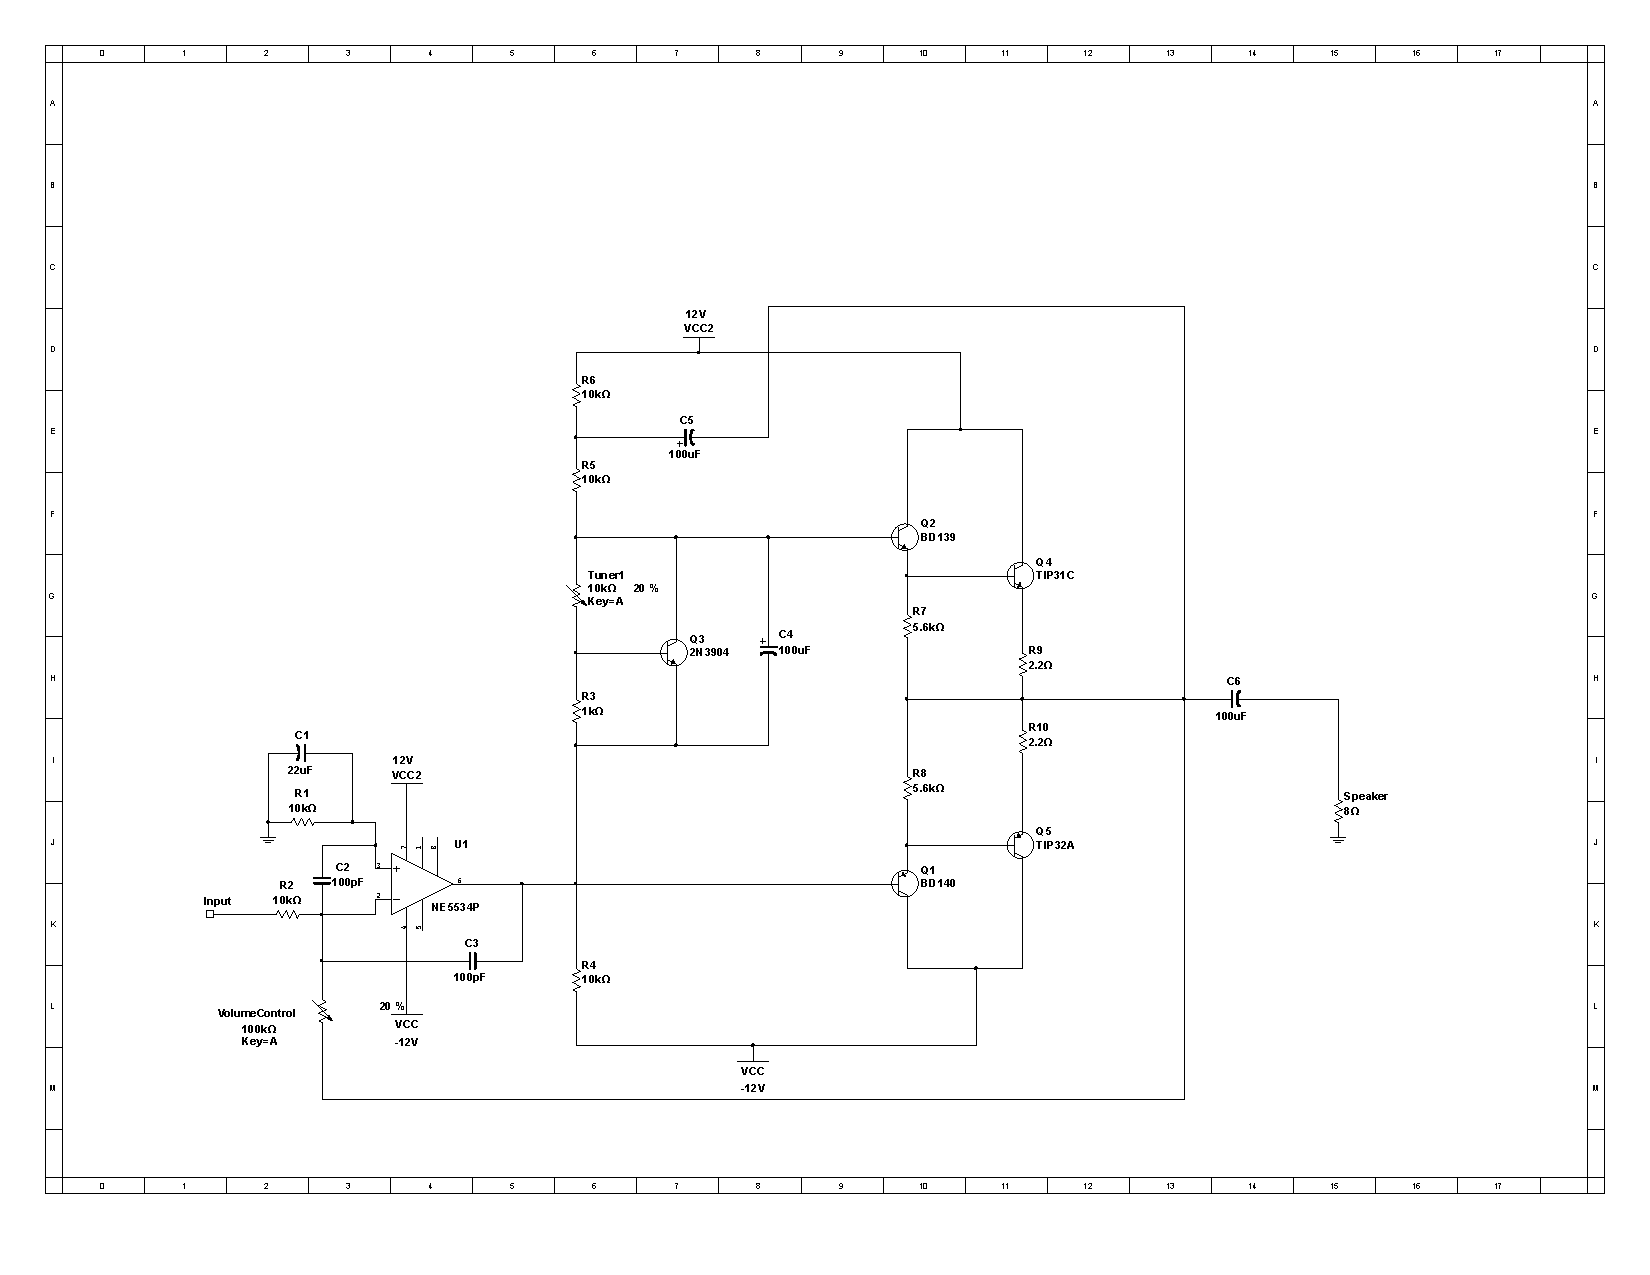
\includegraphics[width=.85\textwidth]{amplifier_mul}
\end{figure}
\newpage

\section{Layout}
\begin{figure}[h]
    
    \begin{subfigure}{\textwidth}
        \centering
        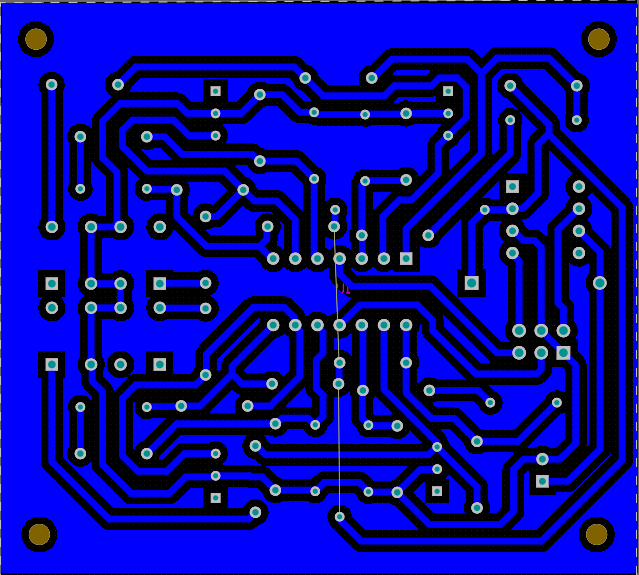
\includegraphics[width=.55\textwidth]{osc_lay}
        \caption{\textbf{PCB-I} : Wave Generator}
    \end{subfigure}
    \vspace*{.5cm}
    \begin{subfigure}{\textwidth}
        \centering
        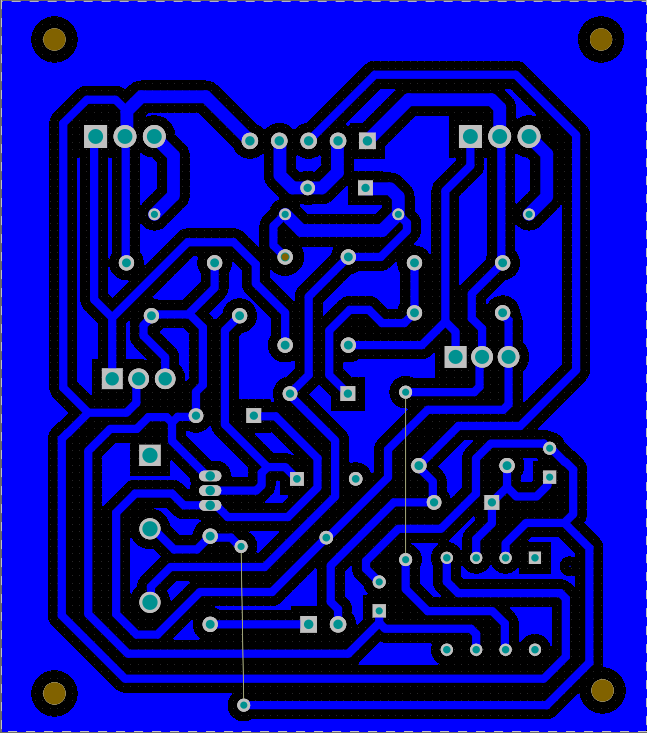
\includegraphics[width=.45\textwidth]{amp_lay}
        \caption{\textbf{PCB-II} : Amplifier}
    \end{subfigure}
\end{figure}
\section{Datasheet}
The datasheet of the model is as follows...
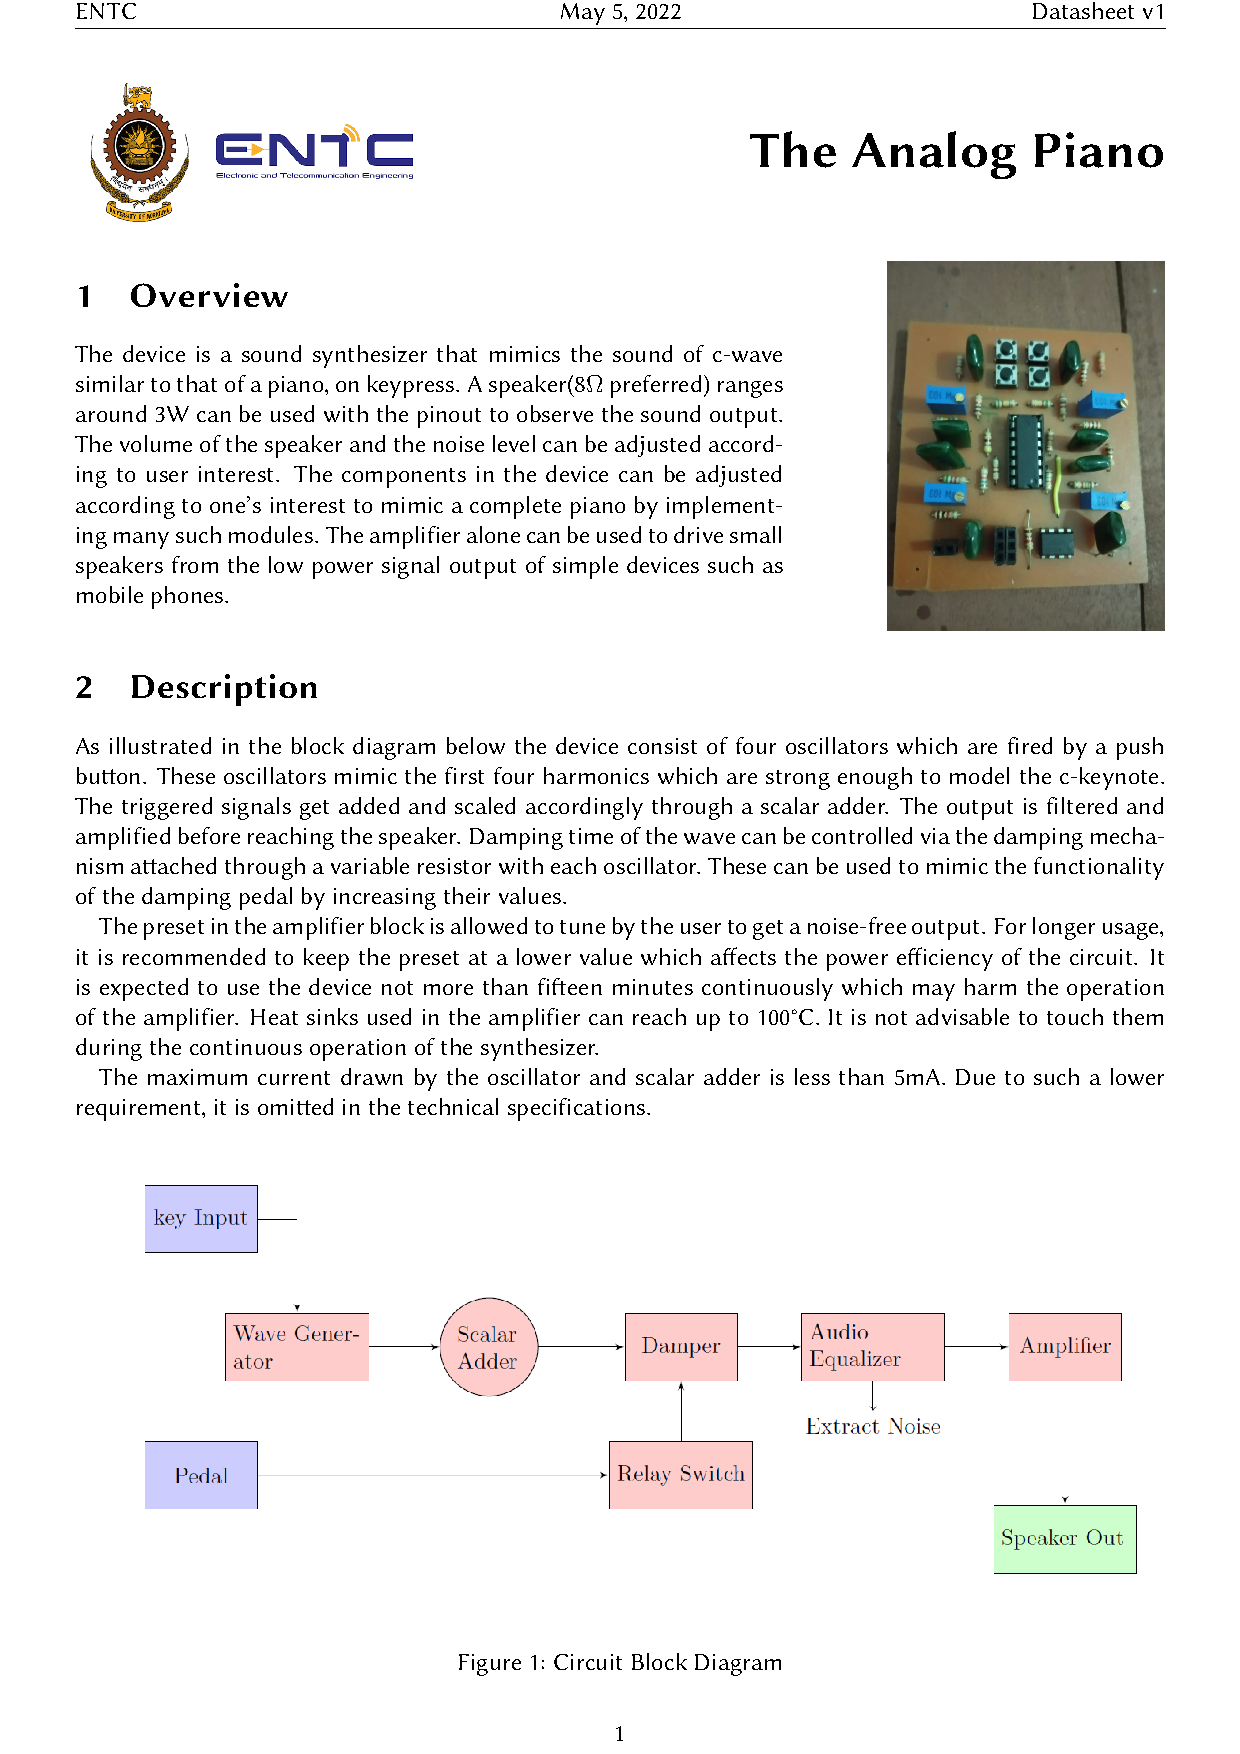
\includepdf[pages=-]{sections/datasheet}
\end{document}